\chapter{Resultados}

\section{Mejoras de eficiencia respecto al prototipo}

Para validar la implementación realizada, se plantean una serie de mediciones comparativas entre instancias computacionales ejecutadas en el prototipo y en \verb|genomus-core| como estimación de las mejoras en eficiencia conseguidas a través de la implementación aportada. 

Se define una instancia de cómputo a realizar iterativamente durante diez segundos. Esta instancia de cómputo consiste en la creación de un vector germinal aleatorio\footnote{Refiriéndose a los vectores germinales descritos por GenoMus\cite{GenoMus-master}} sobre el cual se realizarán las siguientes transformaciones, todas ellas descritas de la misma manera por GenoMus:

\begin{itemize}
    \item Normalización del vector para representar un genotipo válido.
    \item Transformación del vector normalizado a una expresión en forma de texto.
    \item Obtención de un árbol genotípico o genotipo decodificado a través del parser con la expresión como entrada.
    \item Evaluación del genotipo decodificado en un fenotipo codificado.
    \item Representación del fenotipo codificado como un vector numérico.
\end{itemize}

En términos del prototipo, esta serie de evaluaciones y transformaciones son equivalentes a una llamada a la función \verb|createGenotype|. Las instancias de cómputo en ambos software estarán afectadas por los siguientes parámetros:

\begin{itemize}
    \item \textbf{Funciones de GenoMus a utilizar.} Las funciones GenoMus utilizadas tanto por el prototipo como por \verb|genomus-core| son la intersección de funciones definidas en un software y en otro, asegurando así la equivalencia en coste computacional de las instancias de código. La lista de funciones implementadas utilizada se puede consultar en la tabla \ref{tab:used_functions}.
    
    \item \textbf{Longitud máxima del vector germinal.} Se define una longitud máxima del vector germinal de 256.
    \item \textbf{Tamaño máximo por defecto de listas.} Se define un tamaño por defecto de listas de 256.
    \item \textbf{Profundidad máxima de anidamiento de funciones.} Se define una profundidad máxima de anidamiento de 256.
\end{itemize}

\begin{table}[]
    \centering
    \begin{tabular}{p{4cm} p{5cm}}
        Tipo de salida & Funciones \\ \hline \hline
        eventF & e\_piano, eAutoref \\ \hline
        voiceF & v, vConcatE, vConcatV, vMotif, vMotifLoop, vPerpetuumMobile, vPerpetuumMobileLoop, vAutoref \\ \hline
        scoreF & s, sAddV, sAddS \\ \hline
        noteValueF & n, nRnd \\ \hline
        midiPitchF & m, mRnd \\ \hline
        durationF & d, dRnd \\ \hline
        frequencyF & f, fRnd \\ \hline
        articulationF & a, aRnd \\ \hline
        intensityF & i, iRnd \\ \hline
        quantizedF & q, qRnd \\ \hline
        goldenIntegerF & z, zRnd \\ \hline
        lnoteValueF & ln \\ \hline
        lmidiPitchF & lm \\ \hline
        ldurationF & ld \\ \hline
        lfrequencyF & lf \\ \hline
        larticulationF & la \\ \hline
        lintensityF & li \\ \hline
    \end{tabular}
    \caption{Funciones GenoMus utilizadas en las pruebas de eficiencia.} Las descripciones de estas funciones pueden ser encontradas en las especificaciones de GenoMus\cite{GenoMus}. La implementación exacta de estas en \verb|genomus-core| se puede encontrar en el archivo \textit{function\_library.cpp} del repositorio.
    \label{tab:used_functions}
\end{table}

En la tabla \ref{tab:datos_entorno_test} se puede ver una especificación de las características de la máquina donde se ha llevado a cabo la ejecución. Podemos anotar que tanto el prototipo\footnote{
    NodeJS es monohebra a pesar de soportar programación asíncrona. Más información sobre el ciclo de eventos de NodeJS en el siguiente artículo. \url{https://nodejs.org/en/docs/guides/event-loop-timers-and-nexttick/}
} como \verb|genomus-core| no hacen uso de procesamiento paralelo, por lo que la ejecución recae sobre un solo núcleo en cada instante de tiempo.

Como podemos observar en los resultados obtenidos, expuestos en la tabla \ref{tab:resultados_benchmark}, podemos decir que \verb|genomus-core| es aproximadamente cinco veces más rápido que GenoMus en este tipo de instancia de cómputo. Así, se puede decir que el proyecto cumple su objetivo principal. Estos benchmarks han sido ejecutados sobre el MVP de \verb|genomus-core|, por lo que también se puede pensar que hay todavía mucho espacio para la optimización del software.

\begin{table}[]
    \centering
    \begin{tabular}{p{4cm} p{7cm}}
        \textbf{CPU} &  \\ \hline \hline
        Modelo & Intel(R) Core(TM) M-5Y10c CPU \\ 
        Arquitectura & x86\_64 \\
        Núcleos físicos & 2 \\
        Núcleos lógicos & 4 \\
        & \\
        \textbf{Sistema Operativo} & \\ \hline \hline
        Distribución & Ubuntu 20.04.4 LTS x86\_64 \\
        Kernel & linux 5.4.0-121-generic \\
        & \\        
        \textbf{NodeJS} & \\ \hline \hline
        Versión de NodeJS & v16.0.0 \\
        & \\
        \textbf{C++} & \\ \hline \hline
        Compilador & g++ (gcc) \\
        Versión & 9.4.0 (Ubuntu 9.4.0-1ubuntu1~20.04.1) \\
        Nivel de optimización & CMAKE\_CXX\_FLAGS\_RELEASE \\
        & (-O3 en gcc)
        
    \end{tabular}
    \caption{Especificaciones del entorno de ejecución.}
    \label{tab:datos_entorno_test}
\end{table}

\begin{table}[h]
    \begin{subtable}[h]{0.45\textwidth}
        \centering
        \begin{tabular}{p{1.5cm} p{1cm} p{1.8cm}}
            t (ms) & i & t\_avg (ms) \\ \hline \hline
            
            10633 & 48 & 221,52 \\ 
            10194 & 62 & 164,42 \\ 
            10554 & 79 & 133,59 \\ 
            13221 & 46 & 287,41 \\ 
            14195 & 57 & 249,04 \\ 
            20244 & 12 & 1687 \\ 
            10011 & 39 & 256,69 \\ 
            10937 & 56 & 195,30 \\ \hline
            99989 & 399 & 250,60 \\ 
            
        \end{tabular}
       \caption{GenoMus}
       \label{tab:genomus_benchmark}
    \end{subtable}
    \hfill
    \begin{subtable}[h]{0.45\textwidth}
        \centering
        \begin{tabular}{p{1.5cm} p{1cm} p{1.8cm}}
            t (ms) & i & t\_avg (ms) \\ \hline \hline
            10014 & 176 & 56,90 \\ 
            10056 & 210 & 47,89 \\ 
            10436 & 284 & 36,75 \\ 
            11393 & 160 & 71,21 \\ 
            11452 & 110 & 104,11 \\ 
            10080 & 216 & 46,67 \\ 
            10081 & 288 & 35,00 \\ 
            12145 & 259 & 46,89 \\ \hline
            85657 & 1703 & 50,30 \\ 
        \end{tabular}
       \caption{genomus-core}
       \label{tab:genomus-core_benchmark}
     \end{subtable}
     \caption{Resultados del benchmark.} Podemos ver dos tablas conteniendo respectivamente los resultados del benchmark para GenoMus y \verb|genomus-core|. Las columnas tienen los siguientes significados: \textit{t} representa el tiempo total de computación, \textit{i} representa el número total de iteraciones completadas y \textit{t\_avg} representa el tiempo medio por iteración. La última fila de cada tabla corresponde con los resultados totales a lo largo de las ocho ejecuciones del benchmark para cada software.
     \label{tab:resultados_benchmark}
\end{table}

\section{Completitud del MVP}

En el ámbito de gestión del proyecto, se puede decir que el proceso de desarrollo ha sido exitoso, ya que se ha podido completar el MVP que se buscaba para la fecha prevista. En la figura \ref{fig:jira_num_issues} podemos ver cómo el progreso de historias completadas sigue la pendiente usual de un proyecto de estas características.

\begin{figure}
    \centering
    \centerline{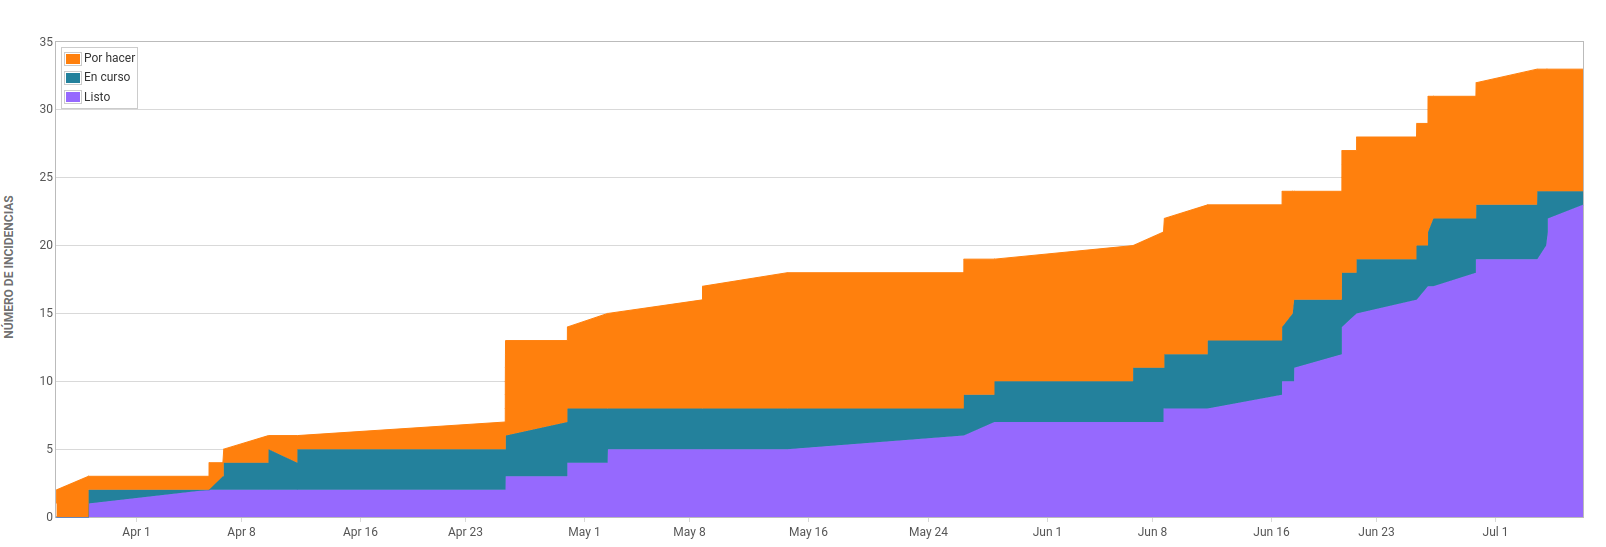
\includegraphics[width=0.8\paperwidth]{imagenes/jira_num_issues.png}}
    \caption{Diagrama de flujo acumulado del progreso en el desarrollo de historias de usuario.} En este diagrama podemos analizar el progreso del desarrollo de las historias de usuario. Las historias no completadas corresponden a funcionalidades no incluidas en el MVP, por lo que quedan pendientes como trabajo futuro.
    \label{fig:jira_num_issues}
\end{figure}